\cleardoublepage

\chapter{Apéndice I}
\label{apendice-i}

Este apéndice reúne el material propio que complementa la memoria pero que, incluido en los
capítulos, habría interrumpido el hilo de la lectura: las tablas con los resultados completos, el
detalle de las pruebas estadísticas y la información necesaria para reproducir el trabajo.

\section{Hiperparámetros completos de los modelos de pronóstico}
\label{apendice-hiperparametros}

Esta sección recoge, con fines de reproducibilidad, el conjunto completo de hiperparámetros de
los tres modelos de pronóstico (TCN, GNN y Transformer geoespacial), tal y como se han fijado en
los \textit{notebooks} de entrenamiento. Para mayor claridad se han separado en dos bloques: los
hiperparámetros de \textbf{arquitectura}, que definen la estructura de cada red
(Tabla~\ref{tab:hiper-arq}), y los de \textbf{entrenamiento}, que controlan el proceso de
optimización (Tabla~\ref{tab:hiper-train}). En el cuerpo de la memoria, la
Tabla~\ref{tab:hiperparametros} resume únicamente los más relevantes.

\begin{table}[ht!]
  \centering
  \small
  \begin{tabular}{@{}lccc@{}}
    \toprule
    \textbf{Hiperparámetro de arquitectura} & \textbf{TCN}                                & \textbf{GNN}  & \textbf{Transformer}     \\
    \midrule
    Características de entrada              & 5                                           & 5             & 5                        \\
    Canales de la TCN                       & (32,32,64,64)                               & (32,32,64)    & (32,32,64)               \\
    Niveles / dilataciones                  & 4 / \{1,2,4,8\}                             & 3 / \{1,2,4\} & 3 / \{1,2,4\}            \\
    Tamaño de \textit{kernel}               & 3                                           & 3             & 3                        \\
    Campo receptivo (días)                  & 61                                          & 29            & 29                       \\
    \textit{Pooling} temporal               & \multicolumn{3}{c}{[último, media, máximo]}                                            \\
    Dim.\ de \textit{embedding} espacial    & ---                                         & 64 (GCN)      & 128 ($D_{\text{model}}$) \\
    Capas espaciales                        & ---                                         & 2 (GCN)       & 2 (codificador)          \\
    Cabezas de atención                     & ---                                         & ---           & 4                        \\
    Dim.\ \textit{feed-forward}             & ---                                         & ---           & 256                      \\
    \textit{Dropout}                        & 0.20                                        & 0.15          & 0.20                     \\
    \bottomrule
  \end{tabular}
  \caption[Hiperparámetros de arquitectura de los modelos de pronóstico]{\textbf{Hiperparámetros de arquitectura} de los tres modelos de pronóstico. El campo receptivo se obtiene de la relación~\eqref{eq:rf-tcn}; todos comparten la misma TCN como bloque temporal y el mismo \textit{pooling} de tres estadísticos.}
  \label{tab:hiper-arq}
\end{table}

\begin{table}[ht!]
  \centering
  \small
  \begin{tabular}{@{}lccc@{}}
    \toprule
    \textbf{Hiperparámetro de entrenamiento} & \textbf{TCN}                                                                  & \textbf{GNN}     & \textbf{Transformer} \\
    \midrule
    Optimizador                              & Adam                                                                          & Adam             & Adam                 \\
    Tasa de aprendizaje inicial              & $3\times10^{-4}$                                                              & $3\times10^{-3}$ & $1\times10^{-4}$     \\
    Tamaño de lote (\textit{batch})          & 64                                                                            & 48               & 32                   \\
    Épocas máximas                           & 80                                                                            & 200              & 200                  \\
    Paciencia (parada temprana)              & 12                                                                            & 6                & 12                   \\
    Decaimiento de pesos ($L_2$)             & $10^{-4}$                                                                     & $10^{-4}$        & $10^{-4}$            \\
    Recorte de gradiente                     & 1.0                                                                           & 1.0              & 1.0                  \\
    Planificador de tasa                     & \multicolumn{3}{c}{\textit{ReduceLROnPlateau} sobre la métrica de validación}                                           \\
    Función de pérdida                       & \multicolumn{3}{c}{entropía cruzada binaria con ponderación de clase}                                                   \\
    Ventana de historia (\textit{lookback})  & 60 d                                                                          & 60 d             & 60 d                 \\
    Ventana de predicción                    & 14 d                                                                          & 30 d             & 30 d                 \\
    Semillas                                 & \multicolumn{3}{c}{\{13, 42, 123, 256, 1024\}}                                                                          \\
    \bottomrule
  \end{tabular}
  \caption[Hiperparámetros de entrenamiento de los modelos de pronóstico]{\textbf{Hiperparámetros de entrenamiento} de los tres modelos de pronóstico. Los tres comparten optimizador, planificador, tipo de pérdida y protocolo multi-semilla; difieren en la tasa de aprendizaje, el tamaño de lote y la duración del entrenamiento.}
  \label{tab:hiper-train}
\end{table}

\section{Validación empírica de la fuente de datos: STEAD frente a USGS}
\label{apendice-stead-usgs}

Una pregunta natural es por qué el pronóstico utiliza el catálogo del USGS y no el dataset STEAD,
que contiene más de un millón de trazas. La razón es que ambos sirven para tareas distintas:
STEAD es una selección curada de formas de onda para entrenar detectores, mientras que el
pronóstico necesita un catálogo \emph{completo} y \emph{homogéneo} en el tiempo. Las
Figuras~\ref{fig:steadcobertura} y~\ref{fig:steadmc} lo demuestran de forma empírica sobre
California.

\begin{figure}[ht!]
  \centering
  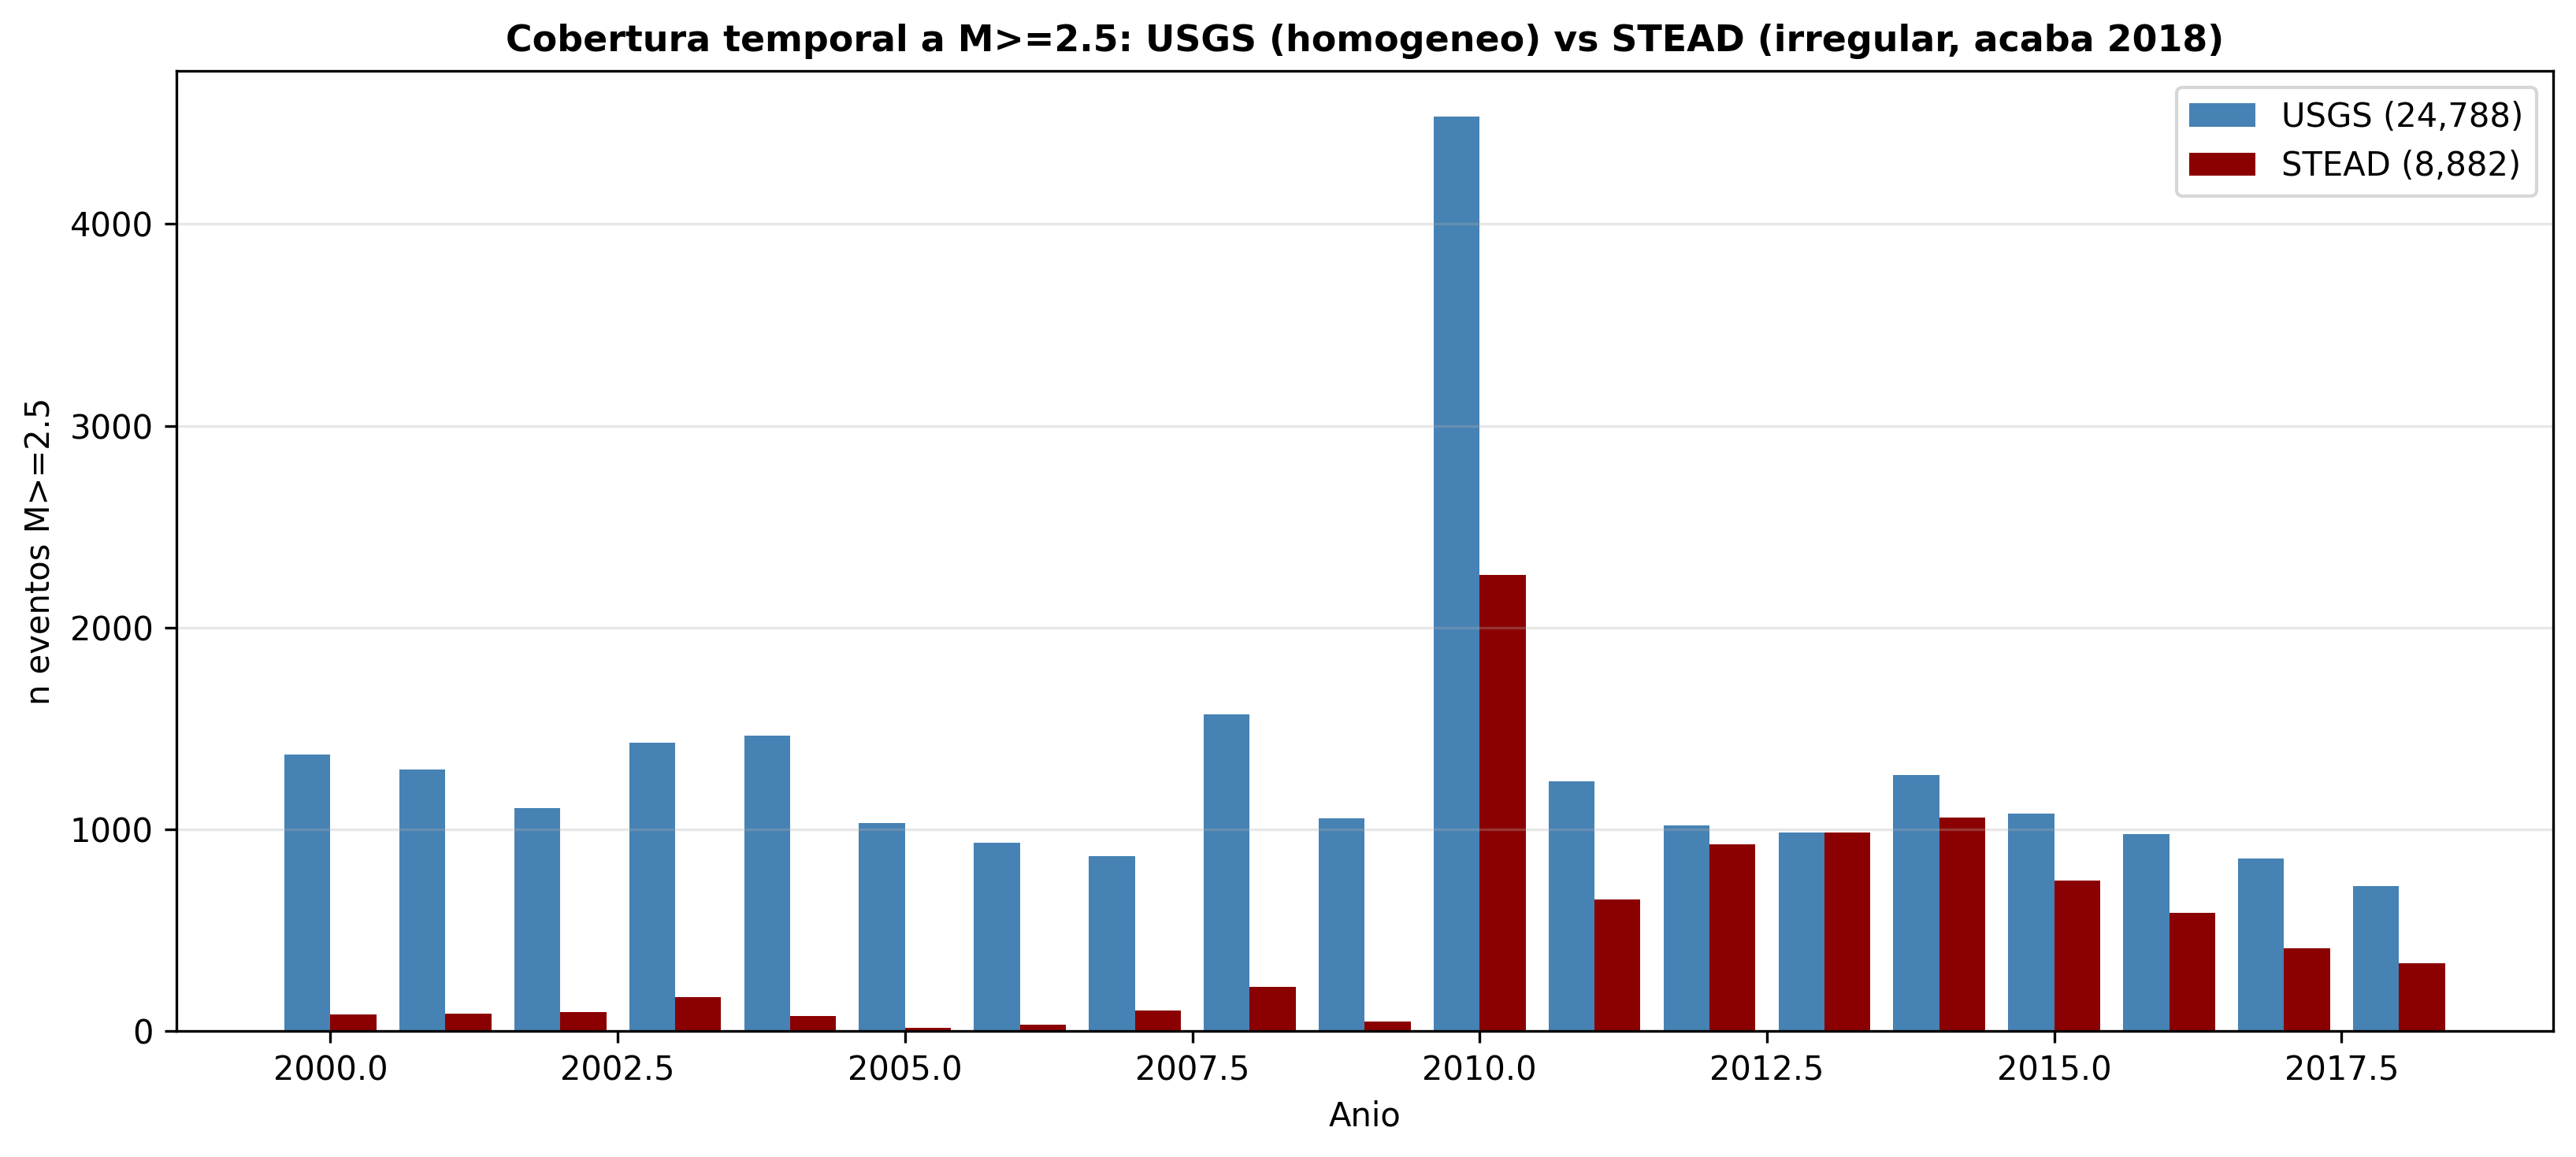
\includegraphics[width=0.92\textwidth]{figuras/07_stead_vs_usgs_cobertura}
  \caption[Cobertura temporal de STEAD frente a USGS]{\textbf{Número de eventos por año (\(M\geq 2.5\)) en California.} El catálogo USGS (azul) ofrece una cobertura continua y homogénea, mientras que STEAD (rojo) presenta un muestreo muy irregular y termina en 2018.}
  \label{fig:steadcobertura}
\end{figure}

\begin{figure}[ht!]
  \centering
  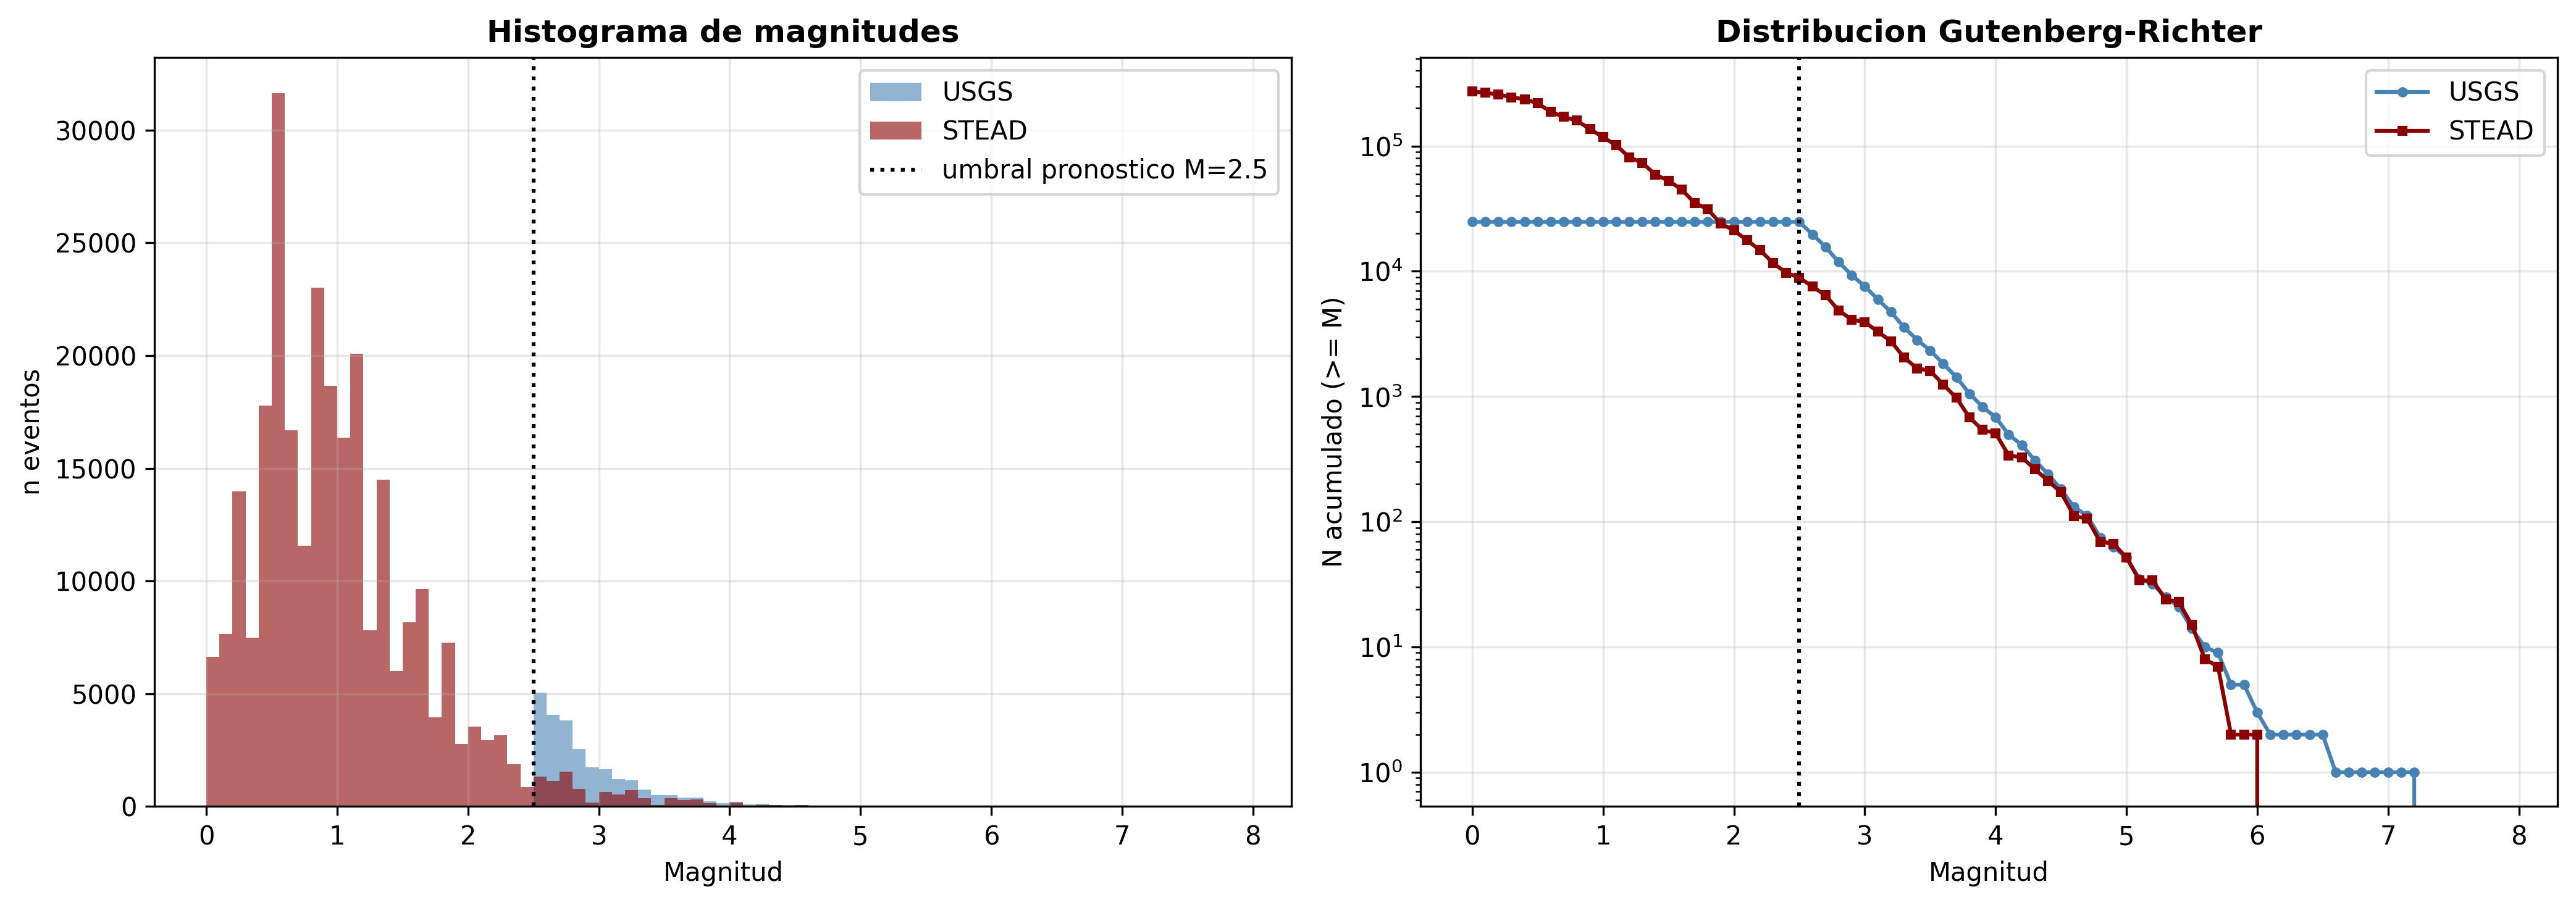
\includegraphics[width=0.92\textwidth]{figuras/07_stead_vs_usgs_magnitud_mc}
  \caption[Distribución de magnitudes y completitud de STEAD frente a USGS]{\textbf{Distribución de magnitudes (izquierda) y curva de Gutenberg--Richter (derecha)} para STEAD y USGS en California. La curva de USGS sigue una recta limpia por encima de la magnitud de completitud, mientras que la de STEAD presenta irregularidades propias de una selección curada.}
  \label{fig:steadmc}
\end{figure}

A igualdad de magnitud (\(M \geq 2.5\)), el USGS contiene en torno a tres veces más eventos que
STEAD en la misma región y periodo, lo que indica que STEAD es incompleto. Su muestreo por año
varía de forma artificial en hasta dos órdenes de magnitud, lo que distorsionaría cualquier
estadística de tasa, y además termina en 2018, por lo que no cubre el periodo de test. Por todo
ello, las características de pronóstico requieren el catálogo USGS, mientras que STEAD se reserva,
con todo su valor, para la fase de detección.

\section{Resultados completos de detección y \textit{picking}}
\label{apendice-deteccion}

La Tabla~\ref{tab:deteccion-completa} amplía la tabla del cuerpo con el rendimiento de PhaseNet y
EQTransformer en las dos fases (P y S) a varias tolerancias temporales, junto con los errores de
localización. Como es esperable, al ampliar la tolerancia mejoran \textit{precision}, \textit{recall}
y \textit{F1}, a costa de un error de localización ligeramente mayor.

\begin{table}[ht!]
  \centering
  \small
  \begin{tabular}{@{}llcccccc@{}}
    \toprule
    \textbf{Modelo} & \textbf{Fase} & \textbf{Tol.\ (s)} & \textbf{Precision} & \textbf{Recall} & \textbf{F1} & \textbf{MAE (s)} & \textbf{RMSE (s)} \\
    \midrule
    PhaseNet        & P             & 0.05               & 0.847              & 0.854           & 0.851       & 0.018            & 0.021             \\
    PhaseNet        & P             & 0.10               & 0.927              & 0.934           & 0.930       & 0.022            & 0.030             \\
    PhaseNet        & P             & 0.20               & 0.957              & 0.965           & 0.961       & 0.026            & 0.039             \\
    PhaseNet        & P             & 0.50               & 0.983              & 0.991           & 0.987       & 0.034            & 0.067             \\
    PhaseNet        & S             & 0.10               & 0.782              & 0.794           & 0.788       & 0.029            & 0.038             \\
    PhaseNet        & S             & 0.20               & 0.879              & 0.892           & 0.885       & 0.042            & 0.060             \\
    PhaseNet        & S             & 0.50               & 0.952              & 0.966           & 0.959       & 0.063            & 0.107             \\
    PhaseNet        & S             & 1.00               & 0.976              & 0.991           & 0.984       & 0.078            & 0.153             \\
    \midrule
    EQTransformer   & P             & 0.05               & 0.736              & 0.656           & 0.694       & 0.018            & 0.024             \\
    EQTransformer   & P             & 0.10               & 0.883              & 0.787           & 0.832       & 0.027            & 0.036             \\
    EQTransformer   & P             & 0.20               & 0.932              & 0.830           & 0.878       & 0.033            & 0.048             \\
    EQTransformer   & P             & 0.50               & 0.957              & 0.853           & 0.902       & 0.040            & 0.072             \\
    EQTransformer   & S             & 0.10               & 0.739              & 0.760           & 0.750       & 0.035            & 0.044             \\
    EQTransformer   & S             & 0.20               & 0.865              & 0.889           & 0.877       & 0.051            & 0.068             \\
    EQTransformer   & S             & 0.50               & 0.943              & 0.969           & 0.956       & 0.073            & 0.115             \\
    EQTransformer   & S             & 1.00               & 0.964              & 0.991           & 0.977       & 0.087            & 0.154             \\
    \bottomrule
  \end{tabular}
  \caption[Resultados completos de detección y \textit{picking}]{\textbf{Detección y \textit{picking} completos} de PhaseNet y EQTransformer sobre STEAD, por fase y tolerancia. MAE y RMSE son los errores de localización de la llegada, en segundos.}
  \label{tab:deteccion-completa}
\end{table}

\section{Métricas operativas completas}
\label{apendice-operativas}

La Tabla~\ref{tab:operativas-completa} detalla las métricas de alerta del Transformer y del Poisson
en los tres niveles de alarma (top 0.5\,\%, 1\,\% y 5\,\%), ampliando las que figuran en el cuerpo.

\begin{table}[ht!]
  \centering
  \small
  \begin{tabular}{@{}lcccccccc@{}}
    \toprule
                       & \multicolumn{2}{c}{\textbf{Top 0.5\,\%}} & \multicolumn{2}{c}{\textbf{Top 1\,\%}} & \multicolumn{2}{c}{\textbf{Top 5\,\%}} & \textbf{PR-AUC} &                                                       \\
    \cmidrule(lr){2-3}\cmidrule(lr){4-5}\cmidrule(lr){6-7}
    \textbf{Métrica}   & \textbf{Trans.}                          & \textbf{Pois.}                         & \textbf{Trans.}                        & \textbf{Pois.}  & \textbf{Trans.} & \textbf{Pois.} & \textbf{Tr./Po.} & \\
    \midrule
    \textit{Precision} & 0.183                                    & 0.160                                  & 0.187                                  & 0.186           & 0.150           & 0.151          & ---              & \\
    \textit{Recall}    & 0.020                                    & 0.018                                  & 0.042                                  & 0.041           & 0.167           & 0.168          & ---              & \\
    \textit{Lift}      & 4.07                                     & 3.56                                   & 4.17                                   & 4.14            & 3.35            & 3.36           & 0.111 / 0.110    & \\
    \bottomrule
  \end{tabular}
  \caption[Métricas operativas completas del Transformer y el Poisson]{\textbf{Métricas operativas completas.} \textit{Precision}, \textit{recall} y \textit{lift} del Transformer (Trans.) y del Poisson (Pois.) en el top 0.5\,\%, 1\,\% y 5\,\% de mayor riesgo, más la PR-AUC.}
  \label{tab:operativas-completa}
\end{table}

\section{Resultados completos de transferencia entre regiones}
\label{apendice-transferencia}

La Tabla~\ref{tab:transferencia-completa} recoge todas las métricas del experimento de
transferencia (Sección~\ref{res-transferencia}) para las nueve regiones evaluadas, incluyendo el
número de celdas activas, los eventos objetivo, la PR-AUC y el \textit{lift}.

\begin{table}[ht!]
  \centering
  \small
  \resizebox{\textwidth}{!}{%
    \begin{tabular}{@{}llcccccccc@{}}
      \toprule
      \textbf{Región}   & \textbf{Continente} & \textbf{$M_c$} & \textbf{Celdas} & \textbf{Objetivos} & \textbf{AUC mod.} & \textbf{AUC Pois.} & \textbf{PR-AUC} & \textbf{Lift@1\%} & \textbf{AUC temp.} \\
      \midrule
      Cascadia (PNW)    & N.\ América         & 2.75           & 31              & 67                 & 0.420             & 0.809              & 0.017           & 0.00              & 0.540              \\
      México (Guerrero) & N.\ América         & 3.95           & 64              & 1125               & 0.538             & 0.600              & 0.255           & 0.95              & 0.517              \\
      Chile norte       & S.\ América         & 4.15           & 155             & 5035               & 0.511             & 0.708              & 0.334           & 0.38              & 0.511              \\
      Perú              & S.\ América         & 4.15           & 45              & 1875               & 0.479             & 0.605              & 0.232           & 0.49              & 0.541              \\
      Italia (Apeninos) & Europa              & 2.75           & 33              & 172                & 0.441             & 0.647              & 0.035           & 1.22              & 0.556              \\
      Grecia (Egeo)     & Europa              & 3.15           & 172             & 1563               & 0.494             & 0.688              & 0.119           & 0.31              & 0.475              \\
      Japón             & Asia                & 4.35           & 188             & 10921              & 0.637             & 0.723              & 0.479           & 1.19              & 0.465              \\
      Sumatra           & Asia                & 4.35           & 94              & 5845               & 0.545             & 0.656              & 0.487           & 1.46              & 0.552              \\
      Magreb            & África              & 2.75           & 17              & 174                & 0.472             & 0.687              & 0.039           & 1.29              & 0.613              \\
      \midrule
      \textbf{Media}    &                     &                &                 &                    & \textbf{0.504}    & 0.671              & 0.222           & 0.81              & 0.530              \\
      \bottomrule
    \end{tabular}}
  \caption[Resultados completos de transferencia entre regiones]{\textbf{Transferencia completa.} Métricas del Transformer (entrenado en California+Alaska) aplicado en inferencia a nueve regiones. En todas, el modelo queda por debajo de su climatología de Poisson local.}
  \label{tab:transferencia-completa}
\end{table}

\section{Contrastes estadísticos}
\label{apendice-estadistica}

La Tabla~\ref{tab:contrastes} reúne las pruebas estadísticas usadas para comparar los modelos. Los
contrastes con la climatología de Poisson son de una muestra (las cinco semillas frente a un valor
escalar); los que comparan dos modelos entrenados usan las cinco semillas comunes, emparejadas.

\begin{table}[ht!]
  \centering
  \small
  \begin{tabular}{@{}llccc@{}}
    \toprule
    \textbf{Comparación}          & \textbf{Test}           & \textbf{Estadístico} & \textbf{\textit{p}-valor} & \textbf{Signif.\ (\(\alpha=0.05\))} \\
    \midrule
    Transformer vs Poisson        & \emph{t}-test 1 muestra & \(t = 2.6\)          & 0.029 (1 cola)            & sí                                  \\
    Transformer vs GNN            & Wilcoxon pareado        & \(W = 0\)            & 0.031 (1 cola)            & sí                                  \\
    Transformer vs GNN            & \emph{t}-test pareado   & \(t = 8.2\)          & 0.001 (2 colas)           & sí                                  \\
    TCN global vs Reg.\ logística & \emph{t}-test 1 muestra & \(t = -3.1\)         & 0.037 (2 colas)           & sí (TCN inferior)                   \\
    \bottomrule
  \end{tabular}
  \caption[Contrastes estadísticos entre modelos]{\textbf{Pruebas estadísticas.} Significancia de las diferencias entre modelos. Con cinco semillas, el Wilcoxon a dos colas no puede bajar de 0.0625, por lo que los contrastes direccionales se reportan a una cola.}
  \label{tab:contrastes}
\end{table}

\section{Entorno de reproducibilidad}
\label{apendice-reproducibilidad}

Para facilitar la reproducción del trabajo se documenta el entorno de ejecución:

\begin{itemize}
  \item \textbf{Cómputo.} Entrenamiento de los modelos en Google Colab con GPU NVIDIA Tesla T4;
        inferencia, evaluación y generación de figuras en CPU local.
  \item \textbf{Lenguaje y librerías.} Python 3.12; \textit{PyTorch} (modelos de aprendizaje
        profundo), \textit{SeisBench} (PhaseNet y EQTransformer preentrenados), \textit{scikit-learn}
        (métricas, regresión logística e isotónica), \textit{SciPy} (procesos gaussianos y tests
        estadísticos), \textit{NumPy}, \textit{pandas} y \textit{Matplotlib}; \textit{tqdm} para la
        monitorización del entrenamiento y \textit{pickle} para la serialización de resultados y
        \textit{checkpoints}.
  \item \textbf{Código y datos.} El código completo (\textit{notebooks} y módulos de \texttt{utils/}),
        junto con el registro experimental, está disponible en el repositorio público
        \url{https://github.com/josecal2844/TFM-Terremotos-Deep-Learning}. El catálogo del USGS se
        descarga a través del \textit{web service} FDSN; las semillas aleatorias están fijadas en el
        conjunto \(\{13, 42, 123, 256, 1024\}\) para garantizar la reproducibilidad.
\end{itemize}
